\documentclass[11pt]{article}
\usepackage{scribe}
\usepackage{amsthm}

\LectureNumber{2}
\LectureDate{May 7th, 2009}
\LectureTitle{Classes of Schedules}

\usepackage{amsmath}
\usepackage{latexsym}
\usepackage{amssymb}
\usepackage{fancybox}
\usepackage{psfig}


\newcommand{\ddate}[1]{\noindent {\marginpar{ \bf #1}} \newline \indent}

\def\ni{\noindent}

\setlength{\oddsidemargin}{0pt}
\setlength{\evensidemargin}{0pt}
\setlength{\textwidth}{6.0in}
\setlength{\topmargin}{0in}
\setlength{\textheight}{8.5in}

\begin{document}
\MakeScribeTop

\section{Classes of Schedules}
A convenient way to visualize schedules is to use what are called {\em block diagrams} or {\em Gantt charts}.
A Gantt chart is a $2$-D plot  with time on the $x$-axis and machines on the $y$-axis. Each job is represented by a series of axis parallel rectangles. Given a schedule $S$, if job $j$ is processed by machine $i$ from time $a_j$ to $b_j$, then there is a rectangle corresponding to job $j$ with $y$-coordinate corresponding to machine $i$, and $x$ coordinates stretching from time $a_j$ to $b_j$. The following example illustrates a Gantt chart.

\begin{example}
Consider the following scheduling problem $(R3~|~prmp~|~\sum C_j)$ with $3$ unrelated parallel machines and $3$ jobs with times as given by the following table.
\begin{center}
\begin{tabular}{|c||c|c|c|}\hline
Jobs & Machine 1 & Machine 2 & Machine 3 \\ \hline
Red & 100 & 100 & 15\\
Blue & 30 & 30 & 10\\
Green & 100 & 15 & 20\\
\hline
\end{tabular}
\end{center}
\vspace{0.1in}
One schedule for the problem runs the {\em blue} job on machine $1$ for $10$ units, on machine $2$ for the next $5$ units and on machine $3$ for the next $5$ units; runs the {\em green} job on machine $2$ for the first $10$ units and then again from time $15$ to time $20$; and runs the {\em red} job on machine $3$ for the first $15$ units. The Gantt chart for this schedule is given as follows.

\begin{figure}[h]
\begin{center}
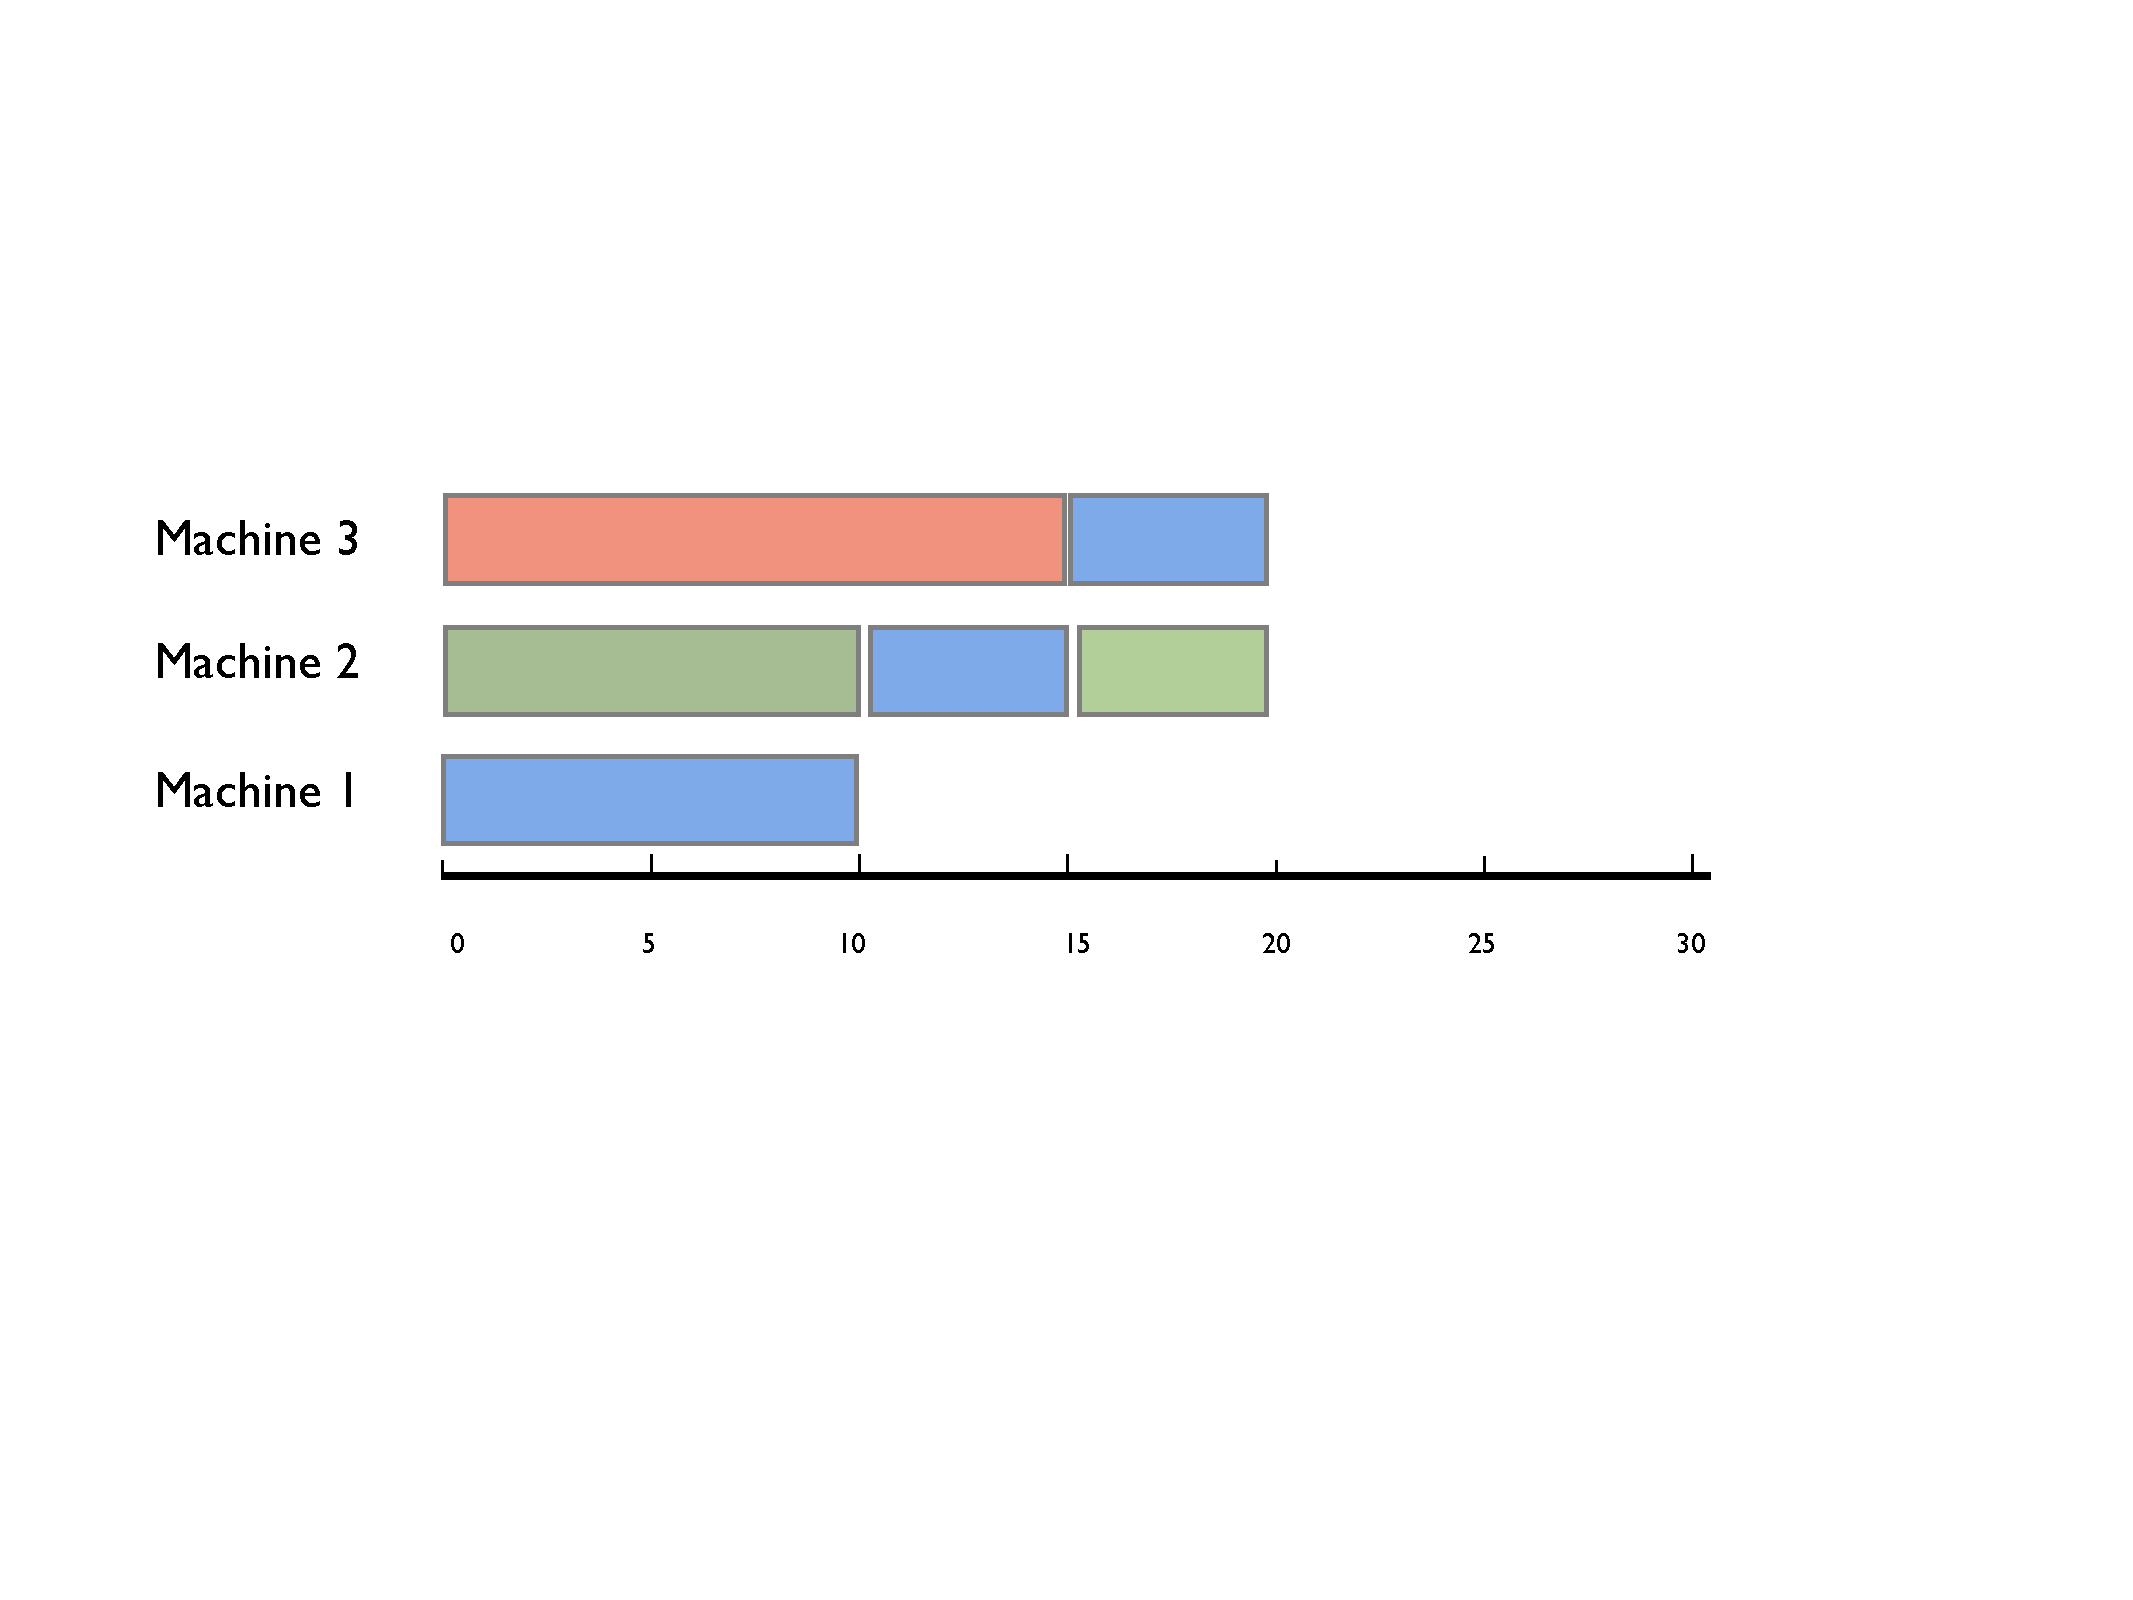
\includegraphics[scale=0.4]{Gantt}
\end{center}
\end{figure}
\end{example} 

We make a few observations about the previous example. Firstly, we note that the above solution is not optimal. The reason is that during time $10$ to $15$, the {\em green} job is not being processed by any machine although machine $1$ is not processing any job in that interval. Thus, a better schedule would be to process some part of the {\em green} job from time $10$ to $15$ on machine $1$, and the the remaining on machine $2$, time $15$ onwards. This decreases $C_{green}$ while keeping the completion time of other jobs the same, thus giving us a better schedule with respect to the performance measure $\sum C_j$. This brings us to the following definition.

\begin{definition} ({\bf Nondelay Schedule}) 
A machine is idle at a time instant if it is not processing any job. 
The idleness is {\em forced} if given the state of the processing of the various jobs, 
no job can be assigned to the machine at that time instant. Otherwise the idleness is called {\em unforced}
A schedule is called nondelay if there is no unforced idleness in the machines at any time instant.
\end{definition}

Let us give an example of forced idleness. Consider an instance of $(P2 ~|~ prec ~|~ \gamma)$ with two jobs with job $1$ preceding job $2$. While job $1$ is being processed on say machine $1$, machine $2$ {\em has} to remain idle till the processing of job $1$ gets completed. This is forced idleness. If there were no precedence constraints, and machine $2$ still remained idle, that would be unforced idleness and the schedule would be a nondelay one.

It might seem from the above example that there is always an optimal schedule which is nondelay. In fact, we show that in some cases that is indeed true, and this brings us to the first theorem of the course.

\begin{theorem}
For any scheduling instance $(\alpha ~|~ prmp, \beta ~|~ \gamma)$ where $\gamma$ is a regular performance measure,
there exists a nondelay schedule which is optimal.
\end{theorem}
\begin{proof}
Although stated as a theorem, this statement actually follows from the definition of nondelay schedules. Consider an optimal schedule $S$ for the problem instance which has some unforced idleness. Therefore, there exists a machine $i$ and a job $j$ and a time instant $t$ when $j$ can be processed but is not processed by any machine, and machine $i$ is idle. Therefore, scheduling a positive fraction of job $j$ on machine $i$ at time $t$, and this can be done since preemption is allowed, decreases the completion time of $j$. Since $\gamma$ is regular, the objective value does not increase. Therefore, we can remove all the unforced idleness in the schedule without increasing its objective value proving there exists an optimal nondelay schedule.
\end{proof}

\begin{exercise}
Show that preemption is necessary for the above theorem. That is, come up with a scheduling problem where no optimal schedule is nondelay. Also show that the regularity condition is necessary for the performance measure. Come up with an example where preemption is allowed, the performance measure is not regular, and no nondelay schedule is optimal.
\end{exercise}

Nondelay schedules can also lead to certain undesirable properties. For instance, given a scheduling problem, one would expect that decreasing the processing time of any job could only decrease the optimum of the scheduling problem. However, we now show an example where the optimal nondelay schedule increases as the processing time of a job is decreased.

\begin{example}
Consider an instance of $(P2 ~|~ prec ~|~ C_{max})$ with $8$ jobs whose processing times are as follows.
\begin{center}
\begin{tabular}{|c||c|c|c|c|c|c|c|c|}\hline
Jobs & 1 & 2 & 3 & 4 & 5 & 6 & 7 & 8 \\ \hline
$p_j$ & 3 & 3 & 3 & 3 & 2 & 2 & 2 & 6\\
\hline
\end{tabular}
\end{center}
\vspace{0.1in}
The precedence constraints are as follows: $1\to 2$; $1\to 3$; $2\to 8$; $3\to 8$; and $5\to 6\to 7\to 8$. 
The optimal schedule is as follows: 
\begin{align*}
\mbox{Machine 1:} ~~ 1 ~~ 2 ~~ 3 ~~ 4 \\
\mbox{Machine 2:} ~~ 5 ~~ 6 ~~ 7 ~~ 8 
\end{align*}
with $C_{max} = 12$. Now consider the example when the processing time of job $7$ goes down to $1$. What is the optimal schedule now? What is the optimal nondelay schedule?
\end{example}

Based on the above examples, we now relax the condition of no unforced idleness to define what is called an active schedule. Recall that a job can consist of various operations and a job is completed only after all the operations is completed.

\begin{definition}
A schedule is called {\em active} if one cannot change the order of processing of operations on the machines and have at least one operation finish earlier and no operation finish later.
\end{definition}

Consider the following scheduling problem. There are three machines and two jobs. Job $1$ needs to be processed on machine $3$ for 
$1$ unit of time and on machine $2$ for $2$ units of time. Job $2$ needs to be processed on machine $2$ for $2$ units of time and on machine $1$ for $2$ units of time. (What is the notation for this scheduling problem?) Consider the following schedule for the problem
given by the Gantt chart. (This example is from the textbook, Page 24).

\begin{figure}[h]
\begin{center}
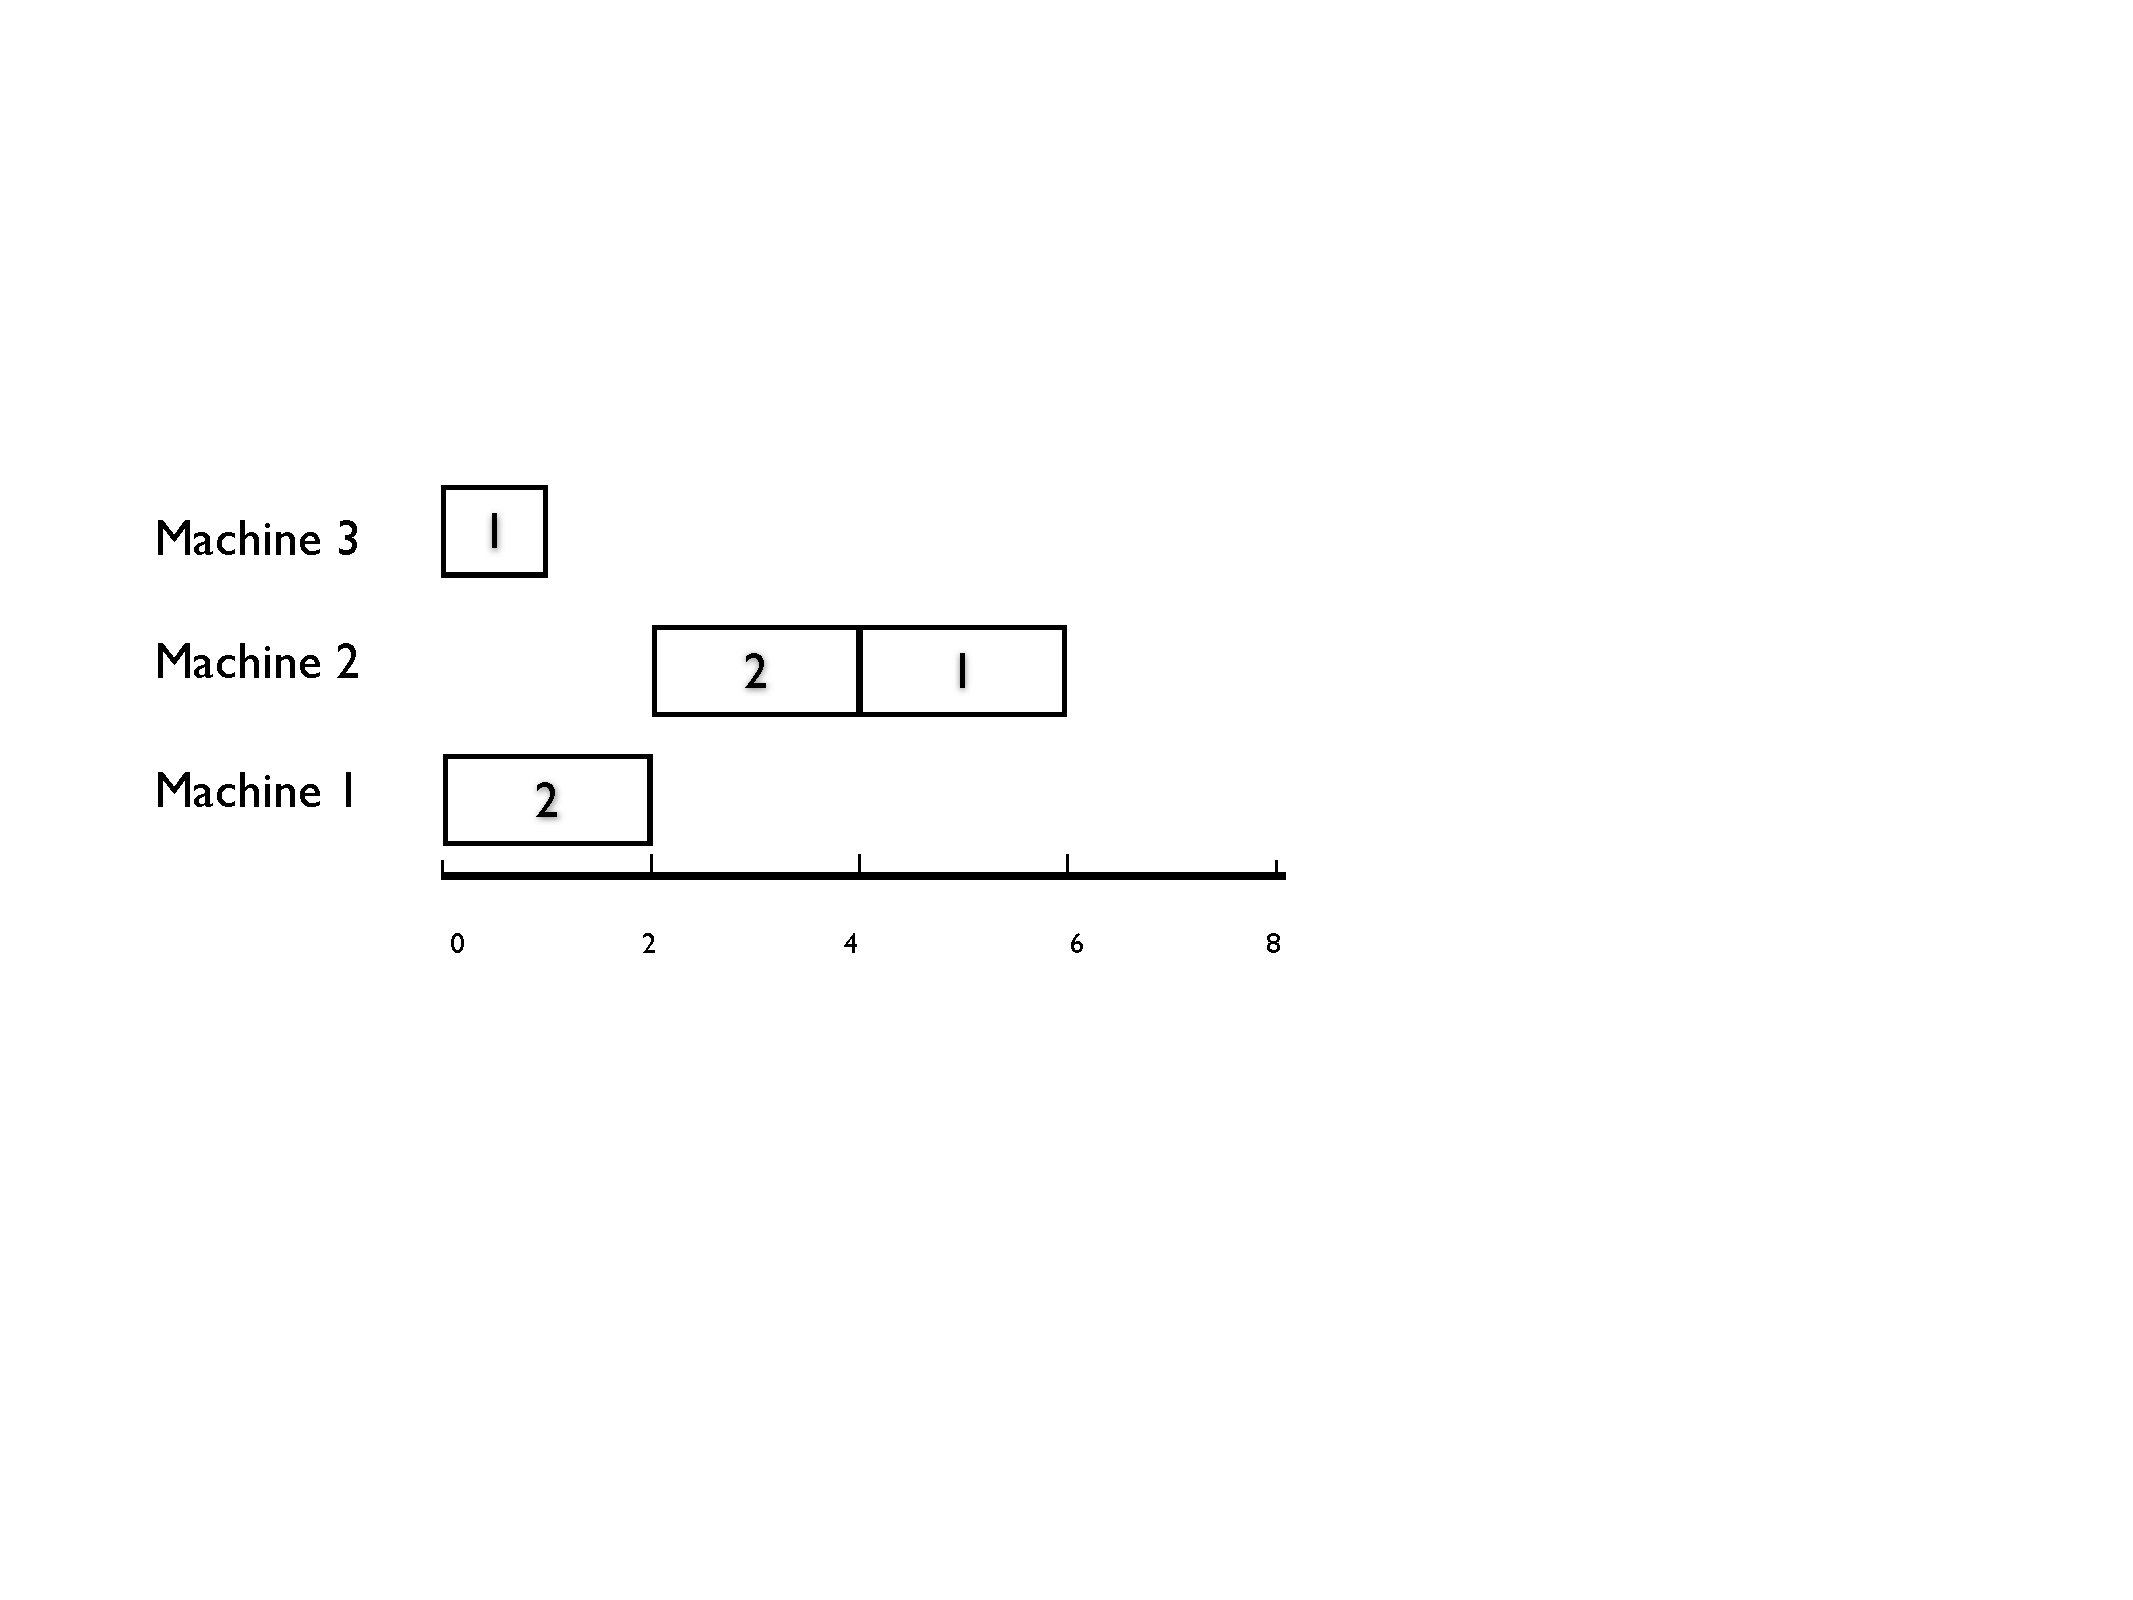
\includegraphics[scale=0.4]{active-schedule}
\end{center}
\end{figure}

The above schedule is active. To see this it suffices to check the order of processing on machine $2$ since it is the only machine which both jobs need processing on. If we process job $1$ before job $2$, note that we can start processing at time $1$ and end by time $3$.
However, job $2$ will end only at time $5$ which is later than the time at which job $2$ finishes in the previous schedule. Note however that the above schedule is not non-delay -- the machine $2$ remains idle between time $1$ and $2$ which job $1$ remains idle as well. 

Now consider a tweak in the problem where we keep everything the same except job $1$ requires time $1$ on machine $2$. The Gantt chart of the above schedule now becomes the following.

\begin{figure}[h]
\begin{center}
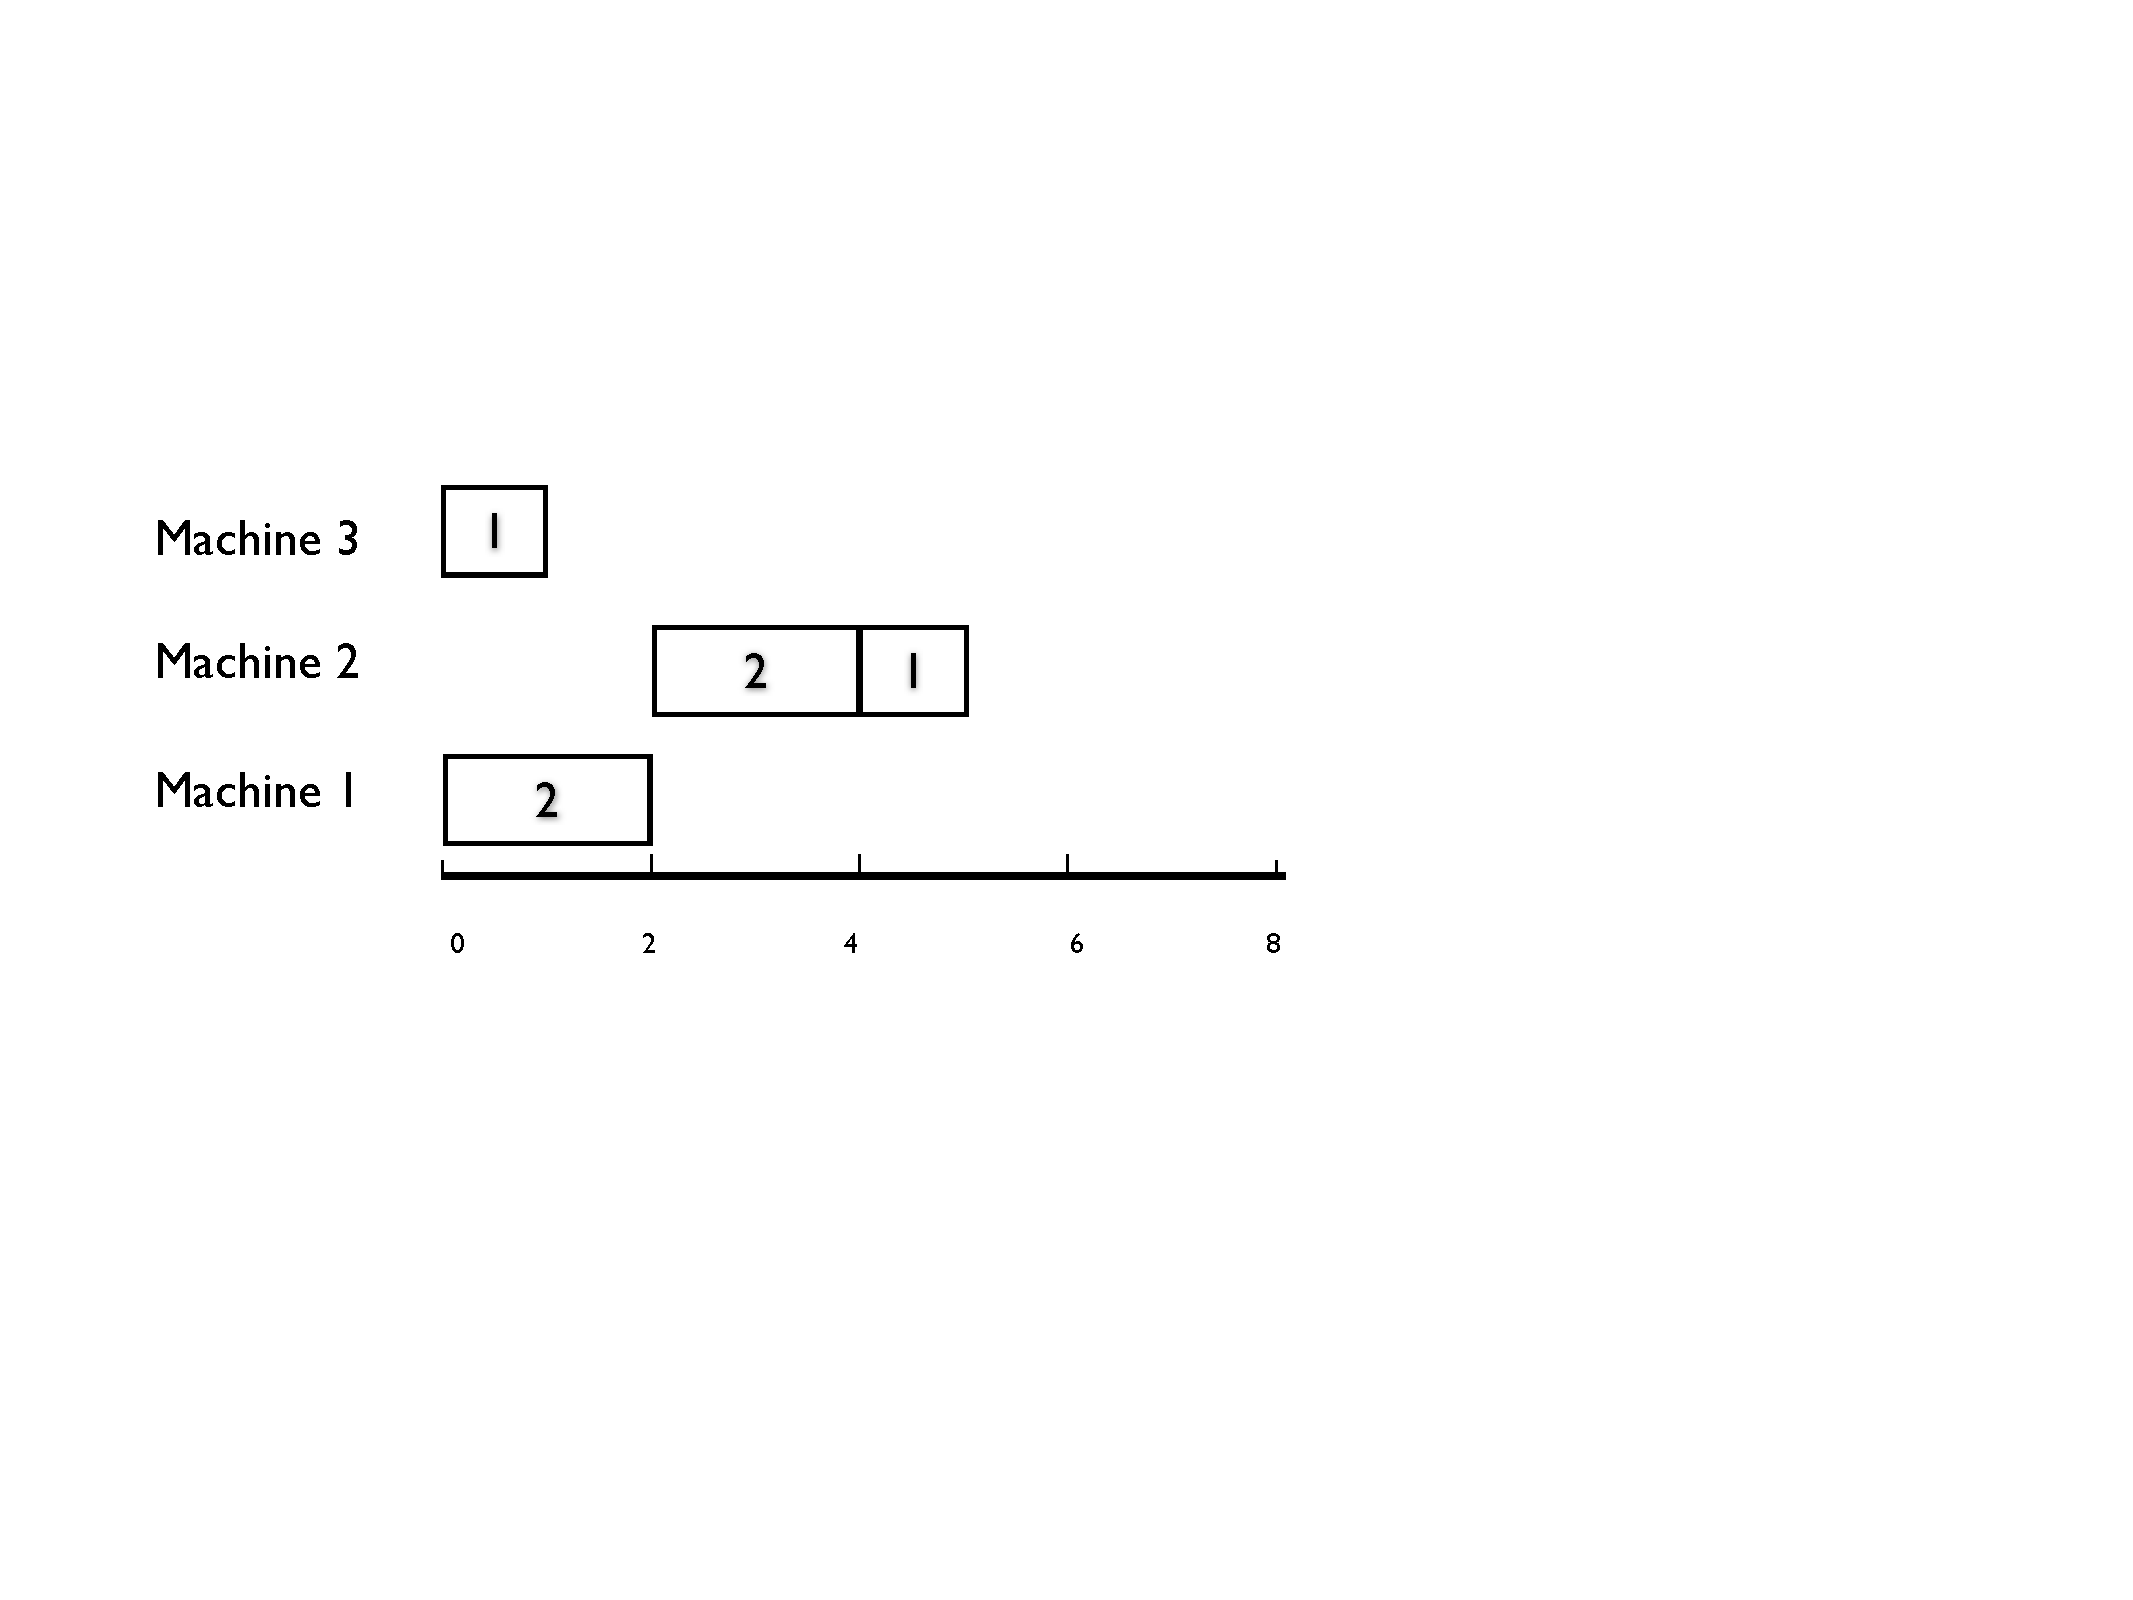
\includegraphics[scale=0.4]{nonactive-schedule}
\end{center}
\end{figure}

The above is {\em not} active because now we can process job $1$ on machine $2$ between times $1$ and $2$ and finish it earlier without changing the completion time of job $2$. 

One way to think of an active schedule is to look at its Gantt chart and claim that one cannot ``fit''  a block corresponding to job $j$ into the ``holes'' appearing to the left of the block, where a holes are time intervals when there is unforced idleness on a machine $i$ with the 
job $j$ being idle at that time as well. Note that in the second example above the rightmost block of job $1$ can be moved into the hole created on machine $2$ from time $1$ to time $2$.

\begin{exercise}
Show that for any regular performance measure $\gamma$, and any problem instance of $(J~|~|~\gamma)$, there exists an active schedule which is optimal. (Note: it is not necessary that all optimal schedules are active).
\end{exercise}

\end{document}